Canada has a long history with nuclear power: the first self-sustained Canadian nuclear reaction was achieved at Chalk River's ZEEP reactor in 1945. Over the years, numerous research reactors and power reactors have been built and decommissioned -- as of 2014, electricity is currently being produced by 19 CANDU reactors in Ontario and New Brunswick. Given that the existence of high energy nuclear waste in Canada is a \emph{fait accompli} -- we have already chosen, as a society, to use nuclear power and create nuclear waste --  it is paramount that we find ways to safely dispose of this waste. 
\par
In 2002, the Nuclear Fuel Waste Act (NFWA) was enacted to study possible strategies for the management of Canada's used nuclear fuel. As a result, the Nuclear Waste Management Organization (NWMO) was established by the Canadian nuclear power companies, with the mandate to provide recommendations to the Canadian Government for the long-term management of used nuclear fuel. One such recommendation, which was accepted in 2007, was the establishment of Adaptive Phased Management (APM) as both a social and technical approach to permanently manage Canada's used nuclear fuel. Canadian citizens determined that the optimal strategy, given the current state of technology in Canada, is the construction of a deep geological repository to contain and isolate the fuel.
\newl
This decision puts the NWMO in a unique and demanding position, as it is the first group in Canada to design and build a unique but extremely performance-critical engineering structure: a long term Canadian repository for high energy nuclear waste. By its very nature, this structure as a whole cannot be tested in advance of use and essentially cannot be maintained once it is built. Furthermore, the environment and materials involved are themselves volatile and their long term behaviour is difficult to predict.
\newl 
Under such challenging circumstances, engineers must do their best to use all of the expertise at their disposal to create as perfect a design as possible for the required structure. Despite the uniqueness of the structure, they need to produce a design that will meet the requirements that have been set out, and then, once built, function exactly as predicted on the first try.  Such a design process is necessarily a lengthy one, involving many designers with high levels of expertise. Many designs would be proposed and rejected before a final design is selected, based on all the evidence and expertise the design team have at their disposal.
\par
At the end of the process the engineering team will have high confidence in the final design that is put forward. The success of the structure in question is critical, and, as responsible, professional engineers, they would not put forward a design for such a structure without being entirely certain, to the best of their collective ability, that this structure will not fail.

Despite this confidence, due diligence requires more than the simple assurance (and belief) from the design team that the structure will not fail. It is not enough, from a societal perspective, for the team to simply provide a ``vote of confidence.'' Rather, due diligence requires the provision of more quantitative information about the failure aspects of the structure. Those responsible for the structure need to be able to determine (and to help the stakeholders understand) what are the structure's necessary and sufficient conditions for failure (and by extension, the conditions for non-failure). To produce these answers they need, in turn, to be able to quantitatively examine what circumstances the structure might encounter, and under these circumstances, what the probability of failure is.

From a testing point of view, the ideal setting would be to build the entire proposed structure many times over and to run trials relating to each of the foreseen circumstances. Data would then be gathered and analyzed to determine the failure tolerance of the structure. Failure probabilities would be calculated based on this data, along with an understanding of possible failure circumstances -- the structure might even be redesigned to take into account the results of the testing. 
\par
However, as we have already noted, this idealistic testing scenario is simply not an option in this case. The structure as a whole cannot be directly tested even once, let alone multiple times. And on top of this, even were many replications of the structure itself available for testing, not all failure circumstances (in particular those involving major geological forces and long time spans) would be possible to re-create in a test environment.
\newl
An alternative strategy is centered around a combination of physical testing and modeling of the behaviour of the structure and environment. More specifically, a larger structure is built up of many component parts, which themselves may be built up of many components. The failure parameters of these component parts may be tested, even if the structure as a whole cannot. \par Similarly, while the structure itself, and perhaps even in some cases the components themselves, cannot be tested repeatedly, there remains the option of creating models of the structure and components in question, and then using the behaviour of these models to predict the behaviour of the components and, in turn, of the structure at large.
\newl
In the absence of the ideal testing scenario, understanding and quantifying the failure of the system as a whole can be carried out by understanding and quantifying the failure circumstances of the components of the system, understanding the causal relationships between these components, creating models of the system as a whole based on these relationships, determine the failure circumstances and probabilities of the constructed structure level model and then transferring these findings over to the structure itself. This results in an estimate of the failure circumstances and probabilities of the actual engineered structure as a whole.
\newl
The end result of this exercise will thus be, rather than a simple yes/no statement (such as ``No, the structure will not fail'', for instance), a list of the possible failure circumstances and an estimate of the failure probabilities for both the structure components and the structure itself, along with a confidence measure indicating a level of confidence in the failure probabilities calculated for each failure circumstance.
\par Such a table of failure circumstances, probabilities, and confidence measures will allow those building the structure to open a legitimate dialogue with those responsible for, and those being affected by, the resulting structure. In essence, this deliverable will allow the designers of the structure to provide their stakeholders with a clearer and more detailed picture of the risks they are likely to encounter when undertaking the construction of such a structure.
\newl 
What steps must be taken to carry out such an exercise, in order to produce what might be referred to as a `Failure Circumstances and Probabilities Table'? Possible required tasks are provided in the Tables found on pp.~\pageref{table:task1}--\pageref{table:task3} in the Tasks section of this proposal. This list of tasks also shows how the expertise and capabilities of statisticians and modelers might fit into the picture of carrying out the larger project of producing such a table.

\paragraph{General Project Objectives} The general objective of this project as a whole is to estimate the failure probability of the Mark II canister and engineered barrier system immediately surrounding the canister. In order to achieve this objective, we will be using a combination of statistical analysis, mathematical modeling, and simulations.
\newl 
More specifically, we will take the approach that our model is meant to answer a specific question, as well as to provide outputs that can be fed into other models, as may be required by already-developed NWMO models. 
\paragraph{The Question to Answer}
The model will be built to answer the following question: \begin{quote}What is the probability that the engineered barrier system (or part(s) thereof) will fail under a particular set of circumstances, taking into account all of the agreed-upon complexities of the barrier system and possible conditions under which it might be placed?\end{quote}
\paragraph{Project's Purposes}
\begin{enumerate}[noitemsep]
\item Existing NWMO models need as an input the probability that the canister and engineered barrier system will fail. Currently, these failure probabilities are estimated  based on relatively simple calculations. However, the NWMO recognizes that greater accuracy in the failure probability estimate for one (or more) canisters is required to appropriately model the ensuing consequences of such failures under varying circumstances.
\item The resulting probabilities are expected to play a role in NWMO's efforts to demonstrate to the licensing agent that interactive failure effects have been considered, not merely failure factors in isolation.
\end{enumerate}

\paragraph{Project Scope} The project's scope (all phases) is defined with respect to several axes:\newl
\textbf{Modeling and Scenarios}\newl
From a physical standpoint, for the overall project, we will model the engineered barrier system and, to a limited extent, the interface between it and the geosphere (rather than the system at large), using a binary fail/non-fail model (rather than a partial failure model). Within this context, we will also look at a reasonable number of scenarios, determined in collaboration with the NWMO..\newl For the Phase 1 Prototype, we shall only consider a specifically selected causal chain. The causal chain will be selected in consultation with subject matter experts; the emphasis of Phase 1 will be on fine-tuning the data gathering and model construction process. \newpage\noindent
\textbf{Analysis}\newl
While CQADS will carry out any and all analyses, we shall rely on the NWMO to gather the relevant data.\newl 
\textbf{Project Coordination}\newl
Our work on this project will interface with other aspects of the NWMO failure test project, but we expect this project to be fairly self-contained in regards to project management and coordination. We will rely on NWMO personnel to assist us in contacting and coordinating with external experts and project members internal to NWMO.\newl
\textbf{Expected Results}\label{sec:to_expect}\newl
For the overall project, we will provide probability failure estimates, along with confidence levels which may depend on the quality of available data (itself depending on the data type, see the Methodology). We will also provide a list of the scenarios that were investigated, as well as a discussion explaining why assessing the probability of failure in the associated circumstances was or was not possible. For the expected results of the Phase 1 Prototype, see Table~\ref{table:phase1tasks}.\newpage\noindent
\textbf{Projects Chain}\label{sec:projects}\newl
With the NWMO's input, the larger project will be divided into a naturally connected chain of smaller projects, keeping in mind which component is being analyzed, and what kind of analysis is used. More details on this structure can be found in Table~\ref{table:prtasks}. 


\paragraph{Project Overview} In the context of the Feasibility Study (December 15, 2014), CQADS presented the NWMO with four project options, the scope of which varied based on the analysis level and system boundaries:  
\begin{itemize}[noitemsep]
\item \textbf{Option I:} analysis of the engineered barrier system (suggested duration: 3.5 years, at 36 hours/week and 48 weeks/year);
\item \textbf{Option II:} analysis of the combined engineered barrier system, and quantitative and qualitative Black Swan Events (suggested duration: 4 years, at 36 hours/week and 48 weeks/year);
\item \textbf{Option III:} analysis of the combined engineered barrier system, quantitative and qualitative Black Swan Events, and Geosphere (suggested duration: 4 years, at 60 hours/week and 48 weeks/year), and
\item \textbf{Option IV:} mix and match analysis, with tasks to be jointly determined by CQADS and the NWMO (suggested duration: to be determined).
\end{itemize}
The suggested tasks corresponding to each option are shown in Tables~\ref{table:task1}--\ref{table:task3}. Tasks of a purely statistical nature have been highlighted in green, those which are mostly about systems modeling in blue, and tasks needing a mixture of approaches in purple; tasks which will need to be completed, but will require the contributions of external personnel (external to the CQADS team) are shown in white. Items have been numbered for reading convenience only; a sequential structure is not necessarily implied, although the item numbers represent natural stop points in the suggested project's progression. \newl The columns ``Project Options'' refer to three streams of project tasks associated with three project options presented in the Project Options, Milestons and Deliverables section; ``Steps'' refers to the four steps identified in the Methodology section (which have been scoped for options I and II only to preserve legibility).  \newl The NWMO has selected Project Option I (see the following section for the identification of the tasks relating to Phase 1: Prototype); the tasks relating to the other options represent a comprehensive possible task list. The tasks for Project Option I can be grouped into 4 phases: \begin{itemize}[noitemsep]
\item Phase 1: Prototype
\item Phase 2: Data Gathering
\item Phase 3: Conceptual Model Creation
\item Phase 4: Simulation/Final Model 
\end{itemize}
\paragraph{Methodology} This section presents a methodology and prototype for a conceptual failure model, which we propose to use and develop in order to carry out a failure probability analysis of the engineered barrier system (i.e., the complete arrangement of engineered barriers that are part of the Deep Geological Repository (DGS), including potentially the wasteform, container, buffer, backfill and shaft seals -- note that the geosphere and access shafts are excluded from this list).\newpage\noindent
The elements of the modeling framework and the expected tasks that will be required to generate these elements are first presented in a general setting; appropriate inputs for the failure model will also be discussed in this context. Additional discussion with respect to the expected source of these inputs and whether or not they are 
\begin{itemize}[noitemsep]
\item likely to be currently available, 
\item will need to be derived during model creation, or 
\item may be difficult or impossible to obtain entirely
\end{itemize}
are also included, as are the likely effects on the failure analysis. 
\newl
The methodology will then be concretely illustrated through the presentation of a conceptual failure model for a very simple sample system, in order to demonstrate the expected inputs, techniques, and outputs at each step of the methodology. While this simple sample system is substantially less complex than the actual system under investigation, our presentation of this simple system will showcase the described methodology, and round out the conceptual failure model prototype.

\subparagraph*{Step 1: Conceptualizing and Analyzing Systems}
\label{sec:methodstep1}
The first steps in the process of creating the failure model involve the accumulation of available information on the engineered barrier system. In that regard, three types of data need to be identified and obtained:
\begin{itemize}[noitemsep]
\item factual-conceptual information about the system components and the properties of these system components;
\item empirical findings from experimental research carried out on system components, and
\item causal information relating to the behaviours of and relationships between system components, with a focus on possible causes of failure of these system components.
\end{itemize}
The first two of these need to be gathered in the first stage of the failure model creation, and then combined to produce a conceptual schema of the system (the third type of information will be discussed in the subsequent section). 
\newl
Gathering the first two data types may require
\begin{itemize}[noitemsep]
\item an identification and listing of system components to be included in the model;
\item a systematic gathering of factual-conceptual information for each of these components and their relationship to connected components (examples of required input include descriptions of the system and components of the system, e.g. design specifications), and
\item stress testing and experimental testing data for each component of the system, with an emphasis on experimental data relating to failure behaviours.
\end{itemize}
Based on the existing literature (see annotated bibliography, Appendix C) and documentation provided by the NWMO, it appears that some information currently exists for the first two types of required data and information; from a feasibility perspective, it should as a result be possible to obtain the information required to generate models through either experimental or theoretical means. \par Carrying out this first step will no doubt further identify any gaps in this required knowledge, which will then have to be filled. Should the available options to fill these identified knowledge gaps prove to be difficult to pursue (for practical reasons), it will most likely still be possible to generate mathematical or simple simulation component behaviour models. \par This approach, however, will come at the cost of decreased confidence in the resulting probability estimate, and consequently should be used sparingly.
\newl Once available data has been gathered, knowledge gaps identified, and (when possible) new data generated, the resulting information can then be abstracted and synthesized into a conceptual schema of the system. This schema will define which objects, object properties, and object relationships are relevant to the failure model, and how these objects, objects properties, and object relationships will be operationalized and concretely represented in the model.
\newl The outputs at this stage of the modeling process will be twofold:
\begin{enumerate}[noitemsep]
\item A table containing
	\begin{itemize}[noitemsep]
	\item a list of the components of the system
	\item for each item in the list:
		\begin{itemize}[noitemsep]
		\item conceptual description of the component;
		\item relevant available experimental/empirical data for each component;
		\item relevant research;
		\item relevant models, and/or
		\item possible ways in which the component may fail.
		\end{itemize}
	\end{itemize}
\item A conceptual schema listing and defining objects, object properties and object relationships, presented in the form of tables and conceptual schematics). See the Section entitled `Illustrating Step 1: Conceptualizing and Analyzing Systems' for examples of these outputs.
% Note to Pat: Need to get references to sections, like the one in the paragraph above to work

\end{enumerate}
\subparagraph{Step 2: Collecting Causal Data}
\label{sec:methodstep2}
The creation of the causal probability model requires one last type of data, namely causal information about the relationships and behaviours of system components, with a focus on possible system events and causes of system failure connected to these events.
\newl
This type of information is connected to the two preceding types in the sense that the first type identifies the objects and properties that exist in the system, the second consists of information about respective individual behaviours of system components under particular circumstances, while the third uses and synthesizes these first two types of information, along with additional known information about the relationships and possible interactions between system components. As a result, any remaining gaps in any one of these types of information should be revealed during the gathering and structuring of this third category.
\newpage\noindent
Failure mode, effects, and criticality analysis (FMECA)/black swan techniques will be applied for generating, eliciting and structuring causal information relating to relationships and behaviours of system components (information from systems experts will be required as input).
\newl Outputs of this stage of the process could be:
\begin{itemize}[noitemsep]
\item a list of direct causal connections between objects within the system;
\item a list of possible failure points within the system as a whole, guided by the conceptual schema created in the preceding stage and the list of direct causal connections, and 
\item a list of possible failure events that may be generated at the interface of the system, where components external to the system interact with the system at defined system boundary points (e.g the engineered barrier system--geosphere boundary)
\end{itemize}

\subparagraph{Step 3: Creating Probabilistic Causal Models}
\label{sec:methodstep3}
With the required system knowledge gathered and conceptualized, the next step in the process is to create one or more probabilistic causal models of the system. The general strategy for this involves creating a directed network of connected events, which reflect the ability of a given event to causally influence the occurrence of another event, or the behaviour of a particular component of the system.
\newl
From a mathematical point of view, this can be further conceptualized by assuming that we are trying to model $J$ canisters in total, and that the state vector for canister $j$ at time $t$ is denoted by $\mathbf{X}_j(t)=(X_{j,1},\ldots,X_{j,k},Y_j)^{\!\top}$, with structure given by an appropriate graph. We further postulate the existence of two time scales: a \textit{reporting time scale}, which is measured in `years', and an interaction time scale, which is measured in `seconds' (`years' and `seconds' may not necessarily correspond to years and seconds, respectively). An easy interpretation for the differing time scales is that  we shall exhibit container failure on the reporting scale $t=0,1,2,\ldots, T$; but the state vector at each $t$ is computed using $N$ intermediate computations at the intermediate scale $\nu=0,\ldots, N$, according to some discrete stochastic dynamical system  
\begin{align}
\label{eq:theds1}
\mathbf{X}^{\nu}_j(t)&=f_j\left(\mathbf{X}_1^{\nu-1}(t),\ldots,\mathbf{X}_1^{0}(t),\dots,\mathbf{X}_j^{\nu-1}(t),\ldots,\mathbf{X}_j^{0}(t),\ldots, \mathbf{X}_J^{\nu-1}(t),\ldots,\mathbf{X}_J^{0}(t); \mathbf{X}_j(t-1),\ldots,\mathbf{X}_j(0);\mathbf{q}_j^{\nu-1}(t)\right) \notag \\ 
\mathbf{X}_j(t+1)&=\mathbf{X}_j^N(t) \\
\mathbf{X}^0_j(t+1)&=\mathbf{X}_j(t+1), \notag
\end{align}
where $\mathbf{q}_j^{\nu-1}(t)$ follows some random joint distribution for each combination of $\nu$ and $t$. \newl 
We can concatenate the state vectors $\mathbf{X}_j(t)$ for all containers to get a system-wide state vector $\mathbf{Z}$ and a system-wide discrete stochastic dynamical system (which may include potential container interactions)
\begin{align}
\label{eq:thedsw}
\mathbf{Z}^{\nu}(t)&=f\left(\mathbf{Z}^{\nu-1}(t),\ldots,\mathbf{Z}^{0}(t); \mathbf{Z}(t-1),\ldots,\mathbf{Z}(0);\mathbf{q}^{\nu-1}(t)\right) \notag \\ 
\mathbf{Z}(t+1)&=\mathbf{Z}^N(t) \\
\mathbf{Z}^0(t+1)&=\mathbf{Z}(t+1), \notag
\end{align}
where $\mathbf{q}^{\nu-1}(t)$ follows some (larger) joint random distribution $\mathcal{D}(t,\nu;\mathbf{w})$ for each combination of $\nu$ and $t$, and some distribution parameter vector $\mathbf{w}$. The critical components of our proposed analysis is to determine the theoretical form of the function $f$ appearing in (\ref{eq:thedsw}) and of the distribution $\mathcal{D}$; we shall seek valid approximations should theoretical considerations be unavailable, or, in the worst case scenario where no causal or modeling information is available, a series of informed simulations.
\newl
There are three main steps involved in creating such a model:
\begin{itemize}[noitemsep]
	\item determine the nodes of the causal network (which reflect objects and events which have causal power)
	\item determine the edges of the causal network (which reflect the connection between direct causes and effects)
	\item determine the properties of the nodes and edges (which reflect properties (e.g. probabilities of failure) of objects and events)
\end{itemize}
Appropriate nodes and edges will reflect what is known about objects and object behaviours (as determined during system conceptualization and analysis) and the cause and effect relationships between these objects (as determined during causal data collection). However, to take into account the difficulties and epistemic limitations inherent in understanding possible causal relationships, additional analysis will be carried out using simple machine learning techniques in order to enable a broader, less biased, exploration of the failure space. This may result in several versions of the causal failure model, each of which will be subjected to the analysis described in the following section.

Determination of the properties of edges and nodes will be further guided by methods developed by Pearl (2000), which are essentially extensions of previous Markovian modeling techniques. Thus the chosen strategy will involve a causal analysis of the system by means of the concepts of necessary, sufficient, and actual causes, along with the concept of counter-factuals, all of which will then be used to create the required causal probability model.

\subparagraph{Step 4: Analyzing Probabilistic Causal Models}
\label{sec:methodstep4}
The resulting causal model will be analyzed using strategies developed by Pearl (2000), along with stochastic modeling techniques and analyses of systems dynamics. The final output of this analysis will be a probability estimate, under specified scenarios, that a given event of interest -- in this case a failure of the barrier system -- may occur, along with additional probability estimates relating to the occurrence of the failure-causing scenarios themselves. 
\newl Each of these estimates will also have associated confidence level metrics, which reflect the level of certainty, and variability, in the probability estimates themselves (see the Section entitled Illustrating the Methodology and Sample Outputs for further details).

\paragraph{Illustrating the Methodology and Sample Outputs}
To briefly illustrate the above methodology elements and steps, it is useful to consider what would be involved in carrying out the failure analysis of (a generalization of) a simple system.
\subparagraph{Simple Sample System Description}
\label{sec:samplesystem_description}

In this case, the illustration system consists of a cylindrical container of liquid surrounded and reinforced by a single band of material circling the container and attached to the container by several rivets (see Figure \ref{fig:container_schematic}). \newl Although this is clearly a relatively trivial system which is abstractly described (\textbf{and so is not to be confused with an actual engineered barrier system model; the probabilities presented here have no link with the reality underpinning the APMRDII design or the DGR}), each of the methodology components described in the preceding sections may be applied to this system, generating an example of the resulting output. In the following sections, we will provide a sample of the expected inputs and outputs required to carry out a failure analysis of this very simple system, resulting in a probability assessment of its failure.
\subparagraph{Illustrating Step 1: Conceptualizing and Analyzing Systems}
\label{sec:step1_illustrate}
After Step 1, two outputs are available: 
\begin{enumerate}[noitemsep] 
\item a table listing the system components and knowledge about those components, along with the source of that knowledge, as illustrated in the case of the simple sample system by Table \ref{table:component_info}, and 
\item a conceptual schema describing the system as it will be represented in the failure model, defined by additional descriptions, tables and diagrams which define the appropriate abstractions and operationalizations, as shown in Figure \ref{fig:container_schematic}).
\end{enumerate}

\begin{table}
\begin{center}
    \begin{tabular}{lll}\Xhline{2\arrayrulewidth}
    \textbf{System Component} & \textbf{Information}                                            & \textbf{Source}          \\
    \Xhline{2\arrayrulewidth}
    container        & constructed of a ductile metal                                           & design specifications     \\
    ~                & initial wall thickness of 3 cm                                                & design specification      \\
    ~                & manufacturing process leads to some                                      & experimental failure data \\
    ~                & \qquad imperfections in the container walls & \\
    ~                & elastic deformation under stress                                         & experimental data         
    \\\hline
    liquid           & density of liquid is 1020kg per meter cubed                              & experimental data         \\
    ~                & reacts with ductile metals                                               & physical materials data   \\
    ~                & produces corrosive compounds when                      & physical materials data   \\
    ~                & \qquad reacting with ductile metals corrodes & \\ 
    ~               &  \qquad ductile metals at a rate dependent on & physical simulation data \\
    ~                & \qquad temperature of liquid and metal & \\ \hline
    reinforcing band & constructed from a semi-brittle compound                         & design specifications     \\
    ~                & has a tensile strength of 2430 MPa                                         & physical materials data   \\
    ~                & brittle fractures under stress                                           & physical materials data    
    
    \\\hline
    rivets           & constructed from semi-brittle metal                                      & design specifications     \\
    ~                & interacts with saline liquids                                            & physical materials data  
\\\hline
    environment     & exerts pressure on system during pressure events                          & physical simulation data 
    \\\Xhline{2\arrayrulewidth}
    \end{tabular}
    \small\caption{Systems components and sources \textbf{(provided solely as an illustration of the methodology)}.}\normalsize
\label{table:component_info}
\end{center}
\end{table}

\begin{figure}%[htbp] %  figure placement: here, top, bottom, or page
   \centering
    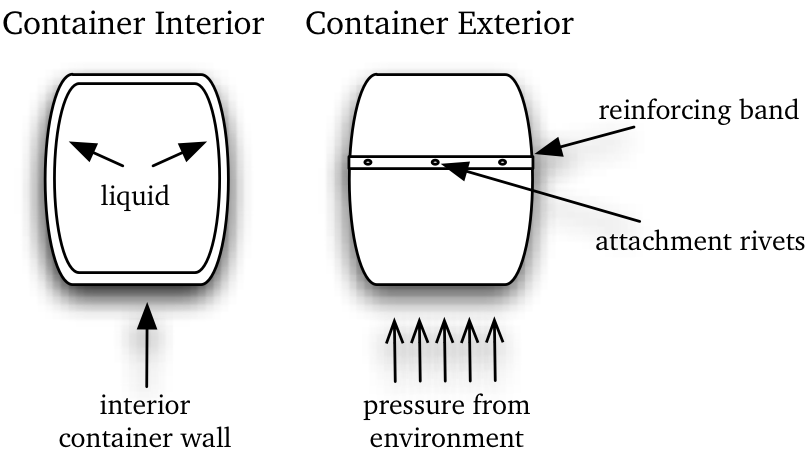
\includegraphics[width=0.6\columnwidth]{images/SIM/container_graphic_smallv3.png} 
   \small\caption[Container conceptual schematic]{Conceptual schematic of the container system \textbf{(provided solely as an illustration of the methodology)}.}\label{fig:container_schematic}\normalsize\hrule
\end{figure}

\begin{table}
\begin{center}
    \begin{tabular}{l l}\Xhline{2\arrayrulewidth}
    \textbf{Components} & \textbf{Component Interaction} \\\Xhline{2\arrayrulewidth}
    liquid, container & the liquid produces pressure on the container.                                                                          \\
 %   liquid, container & There are two chemical reactions taking place due to an interaction between the container \\ & \qquad and the liquid, reaction A and reaction B. \\
    liquid, container & chemical reactions corrode the inner wall  \\ & \qquad of the container at certain rates.                                                              \\
%    liquid, container & Reaction A also produces a product that reduces the speed of corrosion from reaction B, \\  & \qquad relative to the amount that it is produced.   \\
        rivets, reinforcing band & rivets keep reinforcing band tightly attached to container.   \\
        reinforcing band, container & reinforcing band enables container to \\ & \qquad withstand a certain amount of pressure without deforming.   \\ 
        environment, container & when pressure events occur, env. exerts pressure on container system \\ \Xhline{2\arrayrulewidth}
    \end{tabular}
    \small\caption{Component interaction \textbf{(provided solely as an illustration of the methodology)}.}\label{table:system_interactions}\normalsize
\end{center}
\end{table}

%%%%%%%%%%%%%%%%%%%%%%%%%%
% Note to Jen: what gives with all these A and B? Reply from Jen: Okay to leave them commented out
% Note to Pat: I want to add a line to the bottom of the above table, but felt like I was going to mess up the formatting. I'll send you the new line in an e-mail
% From P: ok, got it.
%%%%%%%%%%%%%%%%%%%%%%%%%% 

\begin{table}
\begin{center}
    \begin{tabular}{lll}\Xhline{2\arrayrulewidth}
    \textbf{Failure type}     & \textbf{Failure Category}   & \textbf{Failure}  \\
    \Xhline{2\arrayrulewidth}
    Simple    & Corrosion          & due to corrosion from liquid in container                                                                                                                                                                                                        \\ \hline
    Simple    & Mechanical  & container band snaps/cracks (brittle failure)                                                                                                         \\
    ~                & ~                  & container cracks (probably not happen, assuming a ductile  \\
    ~                & ~                  & \qquad material) \\
    ~                & ~                  & container bursts/ruptures (ductile failure)                                                                                                           \\ \hline
    Compound  & Mechanical  & container deforms $\to$ container bursts                                                                                                                  \\
    ~                & ~                  & pressure on container walls at some point exceed mechanical    \\
    ~                & ~                  & \qquad material  threshold of container wall to resist pressure  \\ 
                     &                    & \qquad  at that point $\to$ container ruptures \\ \Xhline{2\arrayrulewidth}
    \end{tabular}
    \small\caption{Failure types and categories \textbf{(provided solely as an illustration of the methodology)}.}\normalsize\hrule
\label{table:failure_causes}
\end{center}
\end{table}

\subparagraph{Illustrating Step 2: Collecting Causal Data}
Causal Data is collected and stored in two main tables. The first contains information about system interactions, as illustrated by Table \ref{table:system_interactions}. The second (see Table \ref{table:failure_causes}) contains information specifically relating the behaviour of a system component to the failure of another component.
\subparagraph{Illustrating Steps 3 and 4: Creating and Analyzing Probabilistic Causal Models}
The information gathered in the previous steps is then used to create a causal graph, similar to a path diagram (see Figure \ref{fig:causal_graph}). Nodes in the graph represent key events relevant to the failure of the container, which are based on data gathered in preceding steps. Nodes in the causal graph represent states of the system (see Table \ref{table:node_values})
\newl As can be seen in this example, measurements and data from previous stages have been abstracted in a number of ways:	
    \begin{itemize}[noitemsep]
    \item states in the causal model are simple and boolean- i.e. the reinforcing band has either failed or not;
    \item related to the above abstraction, continuous numeric data has been converted to Boolean values relating to failure or non-failure;
    \item underlying chemical and mechanical causes have been subsumed within the system level nodes (e.g. chemical processes affecting container wall thickness are subsumed in nodes $X_1$ and $X_2$; note, however, that this abstraction does not preclude the inclusion of relevant underlying behaviours, as node activation itself can be based on underlying probability models).
    \end{itemize}
As can also be seen from this example, directed edges in the graph represent causal influences between states of specific components of the system -- i.e. if the rivet state becomes one of failure, it can cause the reinforcing band to enter a failure state. By adding in a time component to the graph analysis, these states and state changes can also be interpreted as events -- i.e. the event that rivets in the reinforcing band fail causes the reinforcing band to fail. In this sense, a key aspect of the causal diagram technique is that it allows for the exploration of system behaviours assuming that a particular action has, in fact, occurred. \newl More specifically, although nodes in the graph have initial probabilities based on available data (as described below), it is also possible to assign to each separate node a probability of 1 (i.e. to assume that this event has happened) and then analyze the behaviour of nodes `downstream' from this node based on an occurrence of this event.
\newpage\noindent An analysis of the nodes and edges represented in the graph allows for the calculation of probabilities of failure. The presence of relevant causal interactions, and resulting conditional probabilities can be  derived directly from the structure of the graph. \newl In what follows, $P(A|B)$ can be read as the probability of $A$ occurring given that $B$ is also occurring, or the probability of $A$ occurring in the context of $B$. Looking at the graph, we can see that we should consider the following contextual (conditional) probabilities, based on causal relationships represented in the graph structure:
\begin{itemize}[noitemsep]
\item $P(X_2|X_1)$
\item $P(X_3|X_2)$
\item $P(X_4|X_3)$
\item $P(X_4|X_5)$
\item $P(Y|X_2,X_4,X_5)$
\end{itemize}
Conditional probabilities may then be calculated for each node of the graph by a number of methods, but preferably by abstracting the data gathered in the first stages of the model creation process (see Table \ref{table:sample_experiment_data} for a sketch of this data abstraction). Such calculations provide the context required, along with the conditional probability statements, to calculate and attach to the graph the required probabilities. In the absence of the required experimental data, probability distributions might be used to generate the missing data based on underlying distribution assumptions (for example, assuming that probability of rivet failure follows a Gaussian distribution).
\newl Now consider how the model, in combination with these calculated values, might be used to examine the 3 scenarios described in Table \ref{table:scenarios_description}. With probability values calculated for each conditional probability (see Tables \ref{table:time100_probs}, \ref{table:time1000_probs} and \ref{table:pressure_event_probs}), a stochastic model may be repeatedly run with these values as starting conditions in order to generate an estimate of the probability of container failure.
\begin{figure}[t] %  figure placement: here, top, bottom, or page
   \centering
    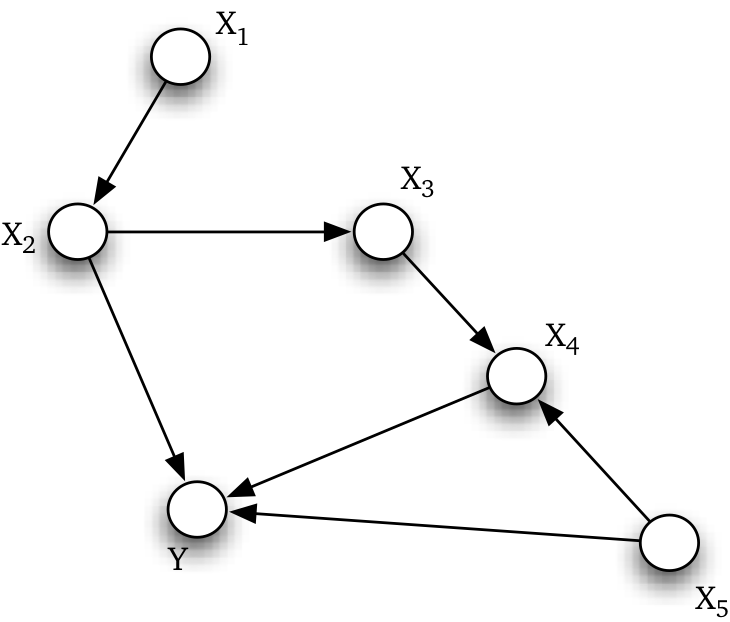
\includegraphics[width=0.4\columnwidth]{images/SIM/methodexamplegraphv3.png} 
   \small\caption[Causal graph]{A direct graph representing the causal model of the container system.}\label{fig:causal_graph}\normalsize\hrule
\end{figure}
\begin{table}
\begin{center}
    \begin{tabular}{cl} \Xhline{2\arrayrulewidth}
        \textbf{Node Label} & \textbf{System State} \\ \Xhline{2\arrayrulewidth}
        $X_1$         &     Thickness   of container wall is 2 mm at some point on the wall \\ 
        $X_2$         &     Thickness   of container wall is 1 mm at some point on the wall \\
        $X_3$         &     One or   more rivets fail                                       \\
        $X_4$         &     Reinforcing   band fails                                        \\
        $X_5$         &     External pressure imposed on container                          \\
        $Y$           & Container fails                                                     \\ \Xhline{2\arrayrulewidth}
    \end{tabular}
        \small\caption{System states and events represented by nodes \textbf{(provided solely as an illustration of the methodology)}.}\normalsize
    \label{table:node_values}
    \end{center}
\end{table}
\begin{table}[htbp]
\begin{center}
    \begin{tabular}{cllllll}\Xhline{2\arrayrulewidth}
     \textbf{Test No.}           & $X_1$ & $X_2$ & $X_3$ & $X_4$ & $X_5$ & $Y$ \\ \Xhline{2\arrayrulewidth}
    Container Test 1   & 1  & 0  & 1  & 0  & 0  & 0 \\
    Container Test 2   & 1  & 1  & 0  & 0  & 0  & 1 \\
    Container Test 3   & 1  & 0  & 1  & 0  & 0  & 1 \\
    $\cdots$              & $\cdots$  & $\cdots$  & $\cdots$  & $\cdots$ & $\cdots$  & $\cdots$ \\ 
    Container Test $M$ & 1  & 1  & 1  & 1  & 1  & 1 \\ \Xhline{2\arrayrulewidth}
    \end{tabular}
            \small\caption{Boolean abstraction of empirical data \textbf{(provided solely as an illustration of the methodology)}.}\normalsize
        \label{table:sample_experiment_data}
\end{center}
\end{table}

%Note to Pat: I changed the text in this table somewhat. I tried to keep the formatting okay, but you should take a look at Scenario 1 to make sure you think it looks okay

\begin{table}[htbp]
\begin{center}
    \begin{tabular}{cl} \Xhline{2\arrayrulewidth}
     \textbf{Scenario Name} & \textbf{Scenario Description} \\ \Xhline{2\arrayrulewidth}
    Scenario 1     & 100 years have passed -- the probability of external pressure imposed on  \\ 
                   & \qquad the container is low. The thickness of the container may become $<$ than 2mm \\\hline
    Scenario 2     & 1000 years have passed but adequate container thickness is maintained \\\hline 
    Scenario 3     & The consequences of an external pressure event having occurred (as represented  \\
                   & \qquad by the probability equalling 1) are explored                                                \\\Xhline{2\arrayrulewidth}
    \end{tabular}
            \small\caption{Three container failure probability scenarios \textbf{(provided solely as an illustration of the methodology)}.}\normalsize
    \label{table:scenarios_description}
    \end{center}
\end{table}
\begin{table}[htbp]
\begin{center}
    \begin{tabular}{cc} \Xhline{2\arrayrulewidth}
     \textbf{Conditional Probability}          & \textbf{Calculated Probability Value at $t=100$} \\\Xhline{2\arrayrulewidth}
    $P(X_1)$                            & 0.003                                     \\
    $P(X_5)$                            & 0.001                                   \\
    $P(X_2|X_1)$                         & 0.007                                   \\
    $P(X_3|X_2)$                         & 0.002                                   \\
    $P(X_4|X_3)$                         & 0.009                                   \\
    $P(X_4|X_5)$                         & 0.002                                   \\
    $P(Y|X_2,X_4,X_5)$                    & 0.009                                   \\ \hline
    Container Failure & $p_{100}$  = 0                                 \\\Xhline{2\arrayrulewidth}
    \end{tabular}
            \small\caption{Conditional probabilities and container failure probability for Scenario 1 \textbf{(provided solely as an illustration of the methodology)}.}\normalsize
    \label{table:time100_probs}
\end{center}
\end{table}
\begin{table}[htbp]
\begin{center}
    \begin{tabular}{cc} \Xhline{2\arrayrulewidth}
     \textbf{Conditional Probability}          & \textbf{Calculated Probability Value at $t=1000$} \\\Xhline{2\arrayrulewidth}
    $P(X_1)$                            & 0                                     \\
    $P(X_5)$                            & 0.001                                   \\
    $P(X_2|X_1)$                         & 0.007                                   \\
    $P(X_3|X_2)$                         & 0.002                                   \\
    $P(X_4|X_3)$                         & 0.009                                   \\
    $P(X_4|X_5)$                         & 0.002                                   \\
    $P(Y|X_2,X_4,X_5)$                    & 0.009                                   \\ \hline
    Container Failure & $p_{1000}$ = 0.6                               \\\Xhline{2\arrayrulewidth}
    \end{tabular}
    \small\caption{Conditional probabilities and container failure probability for Scenario 2 \textbf{(provided solely as an illustration of the methodology)}.}\normalsize
    \label{table:time1000_probs}
    \end{center}
\end{table}
\begin{table}[thbp]
\begin{center}
    \begin{tabular}{cc} \Xhline{2\arrayrulewidth}
     \textbf{Conditional Probability}          & \textbf{Calculated Probability Value at $t= 1000$, event occurs at $t= 990$ } \\ 
     & \textbf{(assuming external pressure event)} \\\Xhline{2\arrayrulewidth}
    $P(X_1)$                            & 0.003                                     \\
    $P(X_5)$                            & 1                                   \\
    $P(X_2|X_1)$                         & 0.007                                   \\
    $P(X_3|X_2)$                         & 0.002                                   \\
    $P(X_4|X_3)$                         & 0.009                                   \\
    $P(X_4|X_5)$                         & 0.002                                   \\
    $P(Y|X_2,X_4,X_5)$                    & 0.009                                   \\ \hline
    Container Failure & $p'_{1000}$ = 0.8                                  \\\Xhline{2\arrayrulewidth}
    \end{tabular}
    \small\caption{Conditional probabilities and container failure probability for Scenario 3 \textbf{(provided solely as an illustration of the methodology)}.}\normalsize
    \label{table:pressure_event_probs}
    \end{center}
\end{table}
\paragraph{Take-Home Points}

As can be seen from this example, the failure analysis of even a simple system requires the careful completion of multiple steps. However, by following these established steps and appropriately abstracting the results of each step prior to proceeding onwards to the following step, a failure probability analysis for the system as a whole can be achieved.

[PAT WILL PUT RELEVANT MATERIAL HERE]

[NOTE WE HAVE A USEFUL VERY SHORT SUMMARY OF THIS PROJECT IN THE CIHI SLIDES]

[ALSO - I HAVE A LITTLE NETLOGO SIMULATION I MADE FOR THIS, SHOWING THE CAUSAL CHAIN FIRING, IF YOU WANT IT FOR DEMO PURPOSES IN YOUR CLASS]

PERHAPS SCREENSHOTS?